The bunch crossing rate at LHC is 40~MHz for a bunch spacing of 25~$\mu$s (about
7 meters), in reality there are several bigger gaps bringing this rate down to
$\approx 31$~MHz. Each event recorded by ATLAS require $\approx 1.4$~MB of disk
space, with approximately 20 to 50 collisions per bunch crossing, the storage
space required to record all the events would be $\approx 60$~TB/s. This is not
feasible thus only the most interesting events are selected and stored on
disk. The \emph{trigger system} decides whether to keep or not a collision event
for later studies, it consists of a hardware based first level trigger (L1) and
a software based high level trigger (HLT).

The L1 trigger determines Region of Interest (RoIs) in the detector using custom
hardware and coarse information from the calorimeter and the muon system. The L1
trigger is capable of reducing the event rate to 100~kHz with a decision time
for a L1 accept of 2.5~$\mu$s. The RoIs from the L1 trigger are sent to the HLT
where different algorithms are run using the full detector information and
reducing the L1 output rate to 1~kHz with a processing time of
200~ms~\cite{trigger}. A schematic overview of the ATLAS trigger and data
acquisition system is shown in Figure~\ref{fig:trigger_system}.

In this analysis the HLT\_xe70 trigger has been used, it receives an L1 accept
that selects events with a missing energy (see
Section~\ref{sec:miss-transv-energy}) greater than 50~GeV, no muons are used in
the reconstruction of the missing energy. At the HLT level, events with a
missing energy greater than 70~GeV are then selected. (\textbf{Are at the HLT
  level the muon used? Otherwise, what's the point of this cut? Couldn't the
  event be selected directly using a 70 GeV cut at L1?})

\begin{figure}[!h]
  \centering
    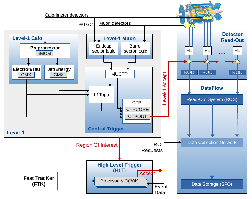
\includegraphics[width=.5\linewidth]{trigger_system}
    \caption{Schematic view of the ATLAS trigger and data acquisition system.}
    \label{fig:trigger_system}
\end{figure}
%%% Local Variables:
%%% mode: latex
%%% TeX-master: "../search_for_DM_LED_with_ATLAS"
%%% End:
